\documentclass[paper=a4, head_space=25mm, foot_space=25mm]{jlreq}

\usepackage{pdfpages}
\usepackage{amsmath}
\usepackage{tabularx, array, booktabs, multirow, makecell}
%tabularx : 表(セル)の幅を自動調節するパッケージ
%array : tabularx環境において中央揃えを可能にするためのパッケージ
%booktabs : 表の罫線の種類を追加するパッケージ
%multirow : 表を縦に結合するパッケージ
%makecell : 表のセル内で改行するためのパッケージ
\usepackage{graphicx, float, subcaption}
%graphicx : 画像を挿入するためのパッケージ
%float : 図を記述した位置通りに表示するためのパッケージ
%subcation : 複数の画像を1つの図として並べて表示させるためのパッケージ
\usepackage[hyphens]{xurl}
%xurl : URLを改行するためのパッケージ
\usepackage[hidelinks]{hyperref}
%hyperref : 目次や参考文献のリンクを有効にするためのパッケージ

\newcolumntype{C}{>{\centering\arraybackslash}X}
%新しい列タイプ"C"を追加 : 幅を自動調節する中央揃えの列

\begin{document}
    \section{目的}
        本実験では、大腸菌からプラスミドを抽出し、そのプラスミドを、同じ複製起点のプラスミドをもつ大腸菌、及び異なる複製起点のプラスミドをもつ大腸菌に加え、形質転換体の数の計測を行った。また、抽出したプラスミドを制限消化し、電気泳動により未処理のプラスミドとの違いを確認した。本実験を通じて、微生物を取り扱う上での基本的な操作と法令、及び形質転換の原理、不和合性、制限修飾系について学んだ。

    \section{方法}
        本節では、プラスミドpMWK1257の抽出、プラスミドpBR322またはpMW118を保有する大腸菌の形質転換、およびプラスミドpMWK1257の制限消化と電気泳動について、これらの実験の手順を述べる。

        \subsection{プラスミドDNAの抽出と精製}
            \subsubsection*{プラスミドpMWK1257の大腸菌からの抽出}
                \begin{enumerate}
                    \item プラスミドpMWK1257を有する\textit{E.coli} DH5 $\alpha$株の一晩培養液 1.5 mLを1.5 mLマイクロチューブに移し、室温、10,000 rpmで1分間だけ遠心した。
                    \item 上清を捨て、チューブに200 $\mu$Lの再懸濁バッファー mP1を加え、ボルテックスで懸濁した。
                    \item チューブに200 $\mu$Lの溶解バッファー mP2を加え、10回ほどゆっくりと転倒混和し、室温で2分間だけ静置した。
                    \item チューブに300 $\mu$Lの中和バッファー mP3を加え、10回ほど転倒混和した。
                    \item チューブを13,000 rpmで5分間だけ遠心した。
                \end{enumerate}
            
            \subsubsection*{抽出したプラスミドpMWK1257の精製}
                \begin{enumerate}
                    \setcounter{enumi}{5}
                    \item FastGene\texttrademark{} mPカラムを2 mLコレクションチューブにセットした。
                    \item 手順5.で得られた上清をmPカラムに移し、13,000 rpmで1分間だけ遠心した。
                    \item mPカラムを一度取り外し、2 mLコレクションチューブに入ったろ液を捨て、カラムをコレクションチューブに再びセットした。
                    \item mPカラムに600 $\mu$Lの洗浄バッファー mP5を加え、13,000 rpmで1分間だけ遠心した。
                    \item 同様にろ液を捨て、再び13,000 rpmで2分間だけ遠心した。
                    \item カラムを新しい1.5 mLマイクロチューブにセットした。
                    \item メンブレンの中央に50 $\mu$Lの溶出バッファー mP6を加え、2分間だけ静置した。
                    \item チューブを13,00 rpmで2分間だけ遠心し、プラスミドを溶出させた。
                    \item 溶出させたプラスミドが入ったチューブを2日目まで保存した。
                \end{enumerate}

        \subsection{大腸菌の形質転換}
            \subsubsection*{プラスミドpBR322またはpMW118を保有するコンピテントセルの作製}
                \begin{enumerate}
                    \item プラスミドpBR322またはpMW118を保有する\textit{E.coli} DH5 $\alpha$株を2時間培養した。
                    \item 各プラスミドを保有する大腸菌の培養液を、1.5 mLずつ別々の1.5 mLマイクロチューブに分注し、4 $^\circ$C、10,000 rpmで1分間だけ遠心した。
                    \item 上清を捨て、菌体が入った各チューブに氷冷した0.1M $\mathrm{CaCl_2}$溶液を1 mLずつ加え、よく懸濁した。
                    \item 各チューブを4 $^\circ$C、10,000 rpmで1分間だけ遠心した。
                    \item 上清を捨て、各チューブに氷冷した10\% グリセリン含有 0.1M $\mathrm{CaCl_2}$溶液を300 $\mu$Lずつ加え、よく懸濁した。
                    \item 各チューブの溶液 300 $\mu$Lのうち、100 $\mu$Lずつを新しい別々のチューブに分注し、残りの溶液 200 $\mu$Lを廃棄した。
                    \item 各チューブを2日目まで-80 $^\circ$Cで保存した。
                \end{enumerate}

            \subsubsection*{コンピテントセルの形質転換と培養}
                \begin{enumerate}
                    \setcounter{enumi}{7}
                    \item 手順1-7.で作製したプラスミドpBR322またはpMW118を保有するコンピテントセルの溶液 100 $\mu$Lに、2.1節で抽出、精製したプラスミドpMWK1257の溶液を5 $\mu$Lずつ加えた。
                    \item 氷中に30分間だけ静置した後、42 $^\circ$Cのヒートブロックに45秒間つけ、その後すぐに氷中で2分間だけ静置した。
                    \item 1 mLのLB培地を各チューブに加え、37 $^\circ$Cで30分間だけ静置培養した。
                    \item 培養後、各形質転換体の培養液を100 $\mu$Lずつ別々のカナマイシン含有LB寒天培地に塗布した。
                    \item 37 $^\circ$Cのインキュベーターで一晩培養した。
                    \item 培養後、各培地を3日目まで4 $^\circ$Cで保存した。
                    \item 3日目に各形質転換体のコロニー数を計測した。
                \end{enumerate}

        \subsection{プラスミドDNAの制限消化}
            \subsubsection*{EcoRIによるプラスミドpMWK1257の制限消化}
                \begin{enumerate}
                    \item 1.5 mLマイクロチューブに、2.1節で抽出、精製したプラスミドpMWK1257の溶液 4 $\mu$Lを加えた。
                    \item チューブに6 $\mu$LのEcoRI酵素溶液を加え、ピペッティングで混和した。
                    \item 37 $^\circ$Cのインキュベーターで10分間だけ静置した。
                \end{enumerate}

            \subsubsection*{電気泳動用プラスミド試料の調製}
                \begin{enumerate}
                    \setcounter{enumi}{3}
                    \item 手順1-3.で作製したEcoRI制限消化済みのプラスミドpMWK1257の溶液 10 $\mu$Lに、6x Loading Buffer Triple Dye 2 $\mu$Lを加えた。
                    \item 続いて、2.1節で抽出、精製した未処理のプラスミドpMWK1257の溶液 4 $\mu$L、水 6 $\mu$L、6x Loading Buffer Triple Dye 2 $\mu$Lをパラフィルム上で混合した。
                \end{enumerate}
            
            \subsubsection*{アガロースゲル電気泳動}
                \begin{enumerate}
                    \setcounter{enumi}{5}
                    \item 手順4-5.で調製した溶液全量と$\lambda$HindⅢ分子量マーカー 4 $\mu$Lを、アガロースゲルの別々のレーンにアプライした。
                    \item 100Vで30分間通電し、電気泳動を行なった。
                    \item 電気泳動後、ゲルをGelRed液で20分間だけ染色した。
                    \item 染色後、ゲルを紫外線イルミネーターで観察したところ、バンドが薄かったため、再度GelRed液で24時間染色した。
                    \item 染色後、ゲルを紫外線イルミネーターで観察した。
                \end{enumerate}

    \section{結果}
        本節では、プラスミドpBR322またはpMW118を保有する大腸菌の形質転換体の培養結果、各形質転換体のコロニー数の解析、およびプラスミドpMWK1257の電気泳動結果について述べる。
        
        \subsection{形質転換体の培養結果}
            以下の図\ref{fig:形質転換体}に、2.2節において形質転換体を培養した培地の写真を示す。
            
            \begin{figure}
                \centering
                \begin{subfigure}{0.49\textwidth}
                    \centering
                    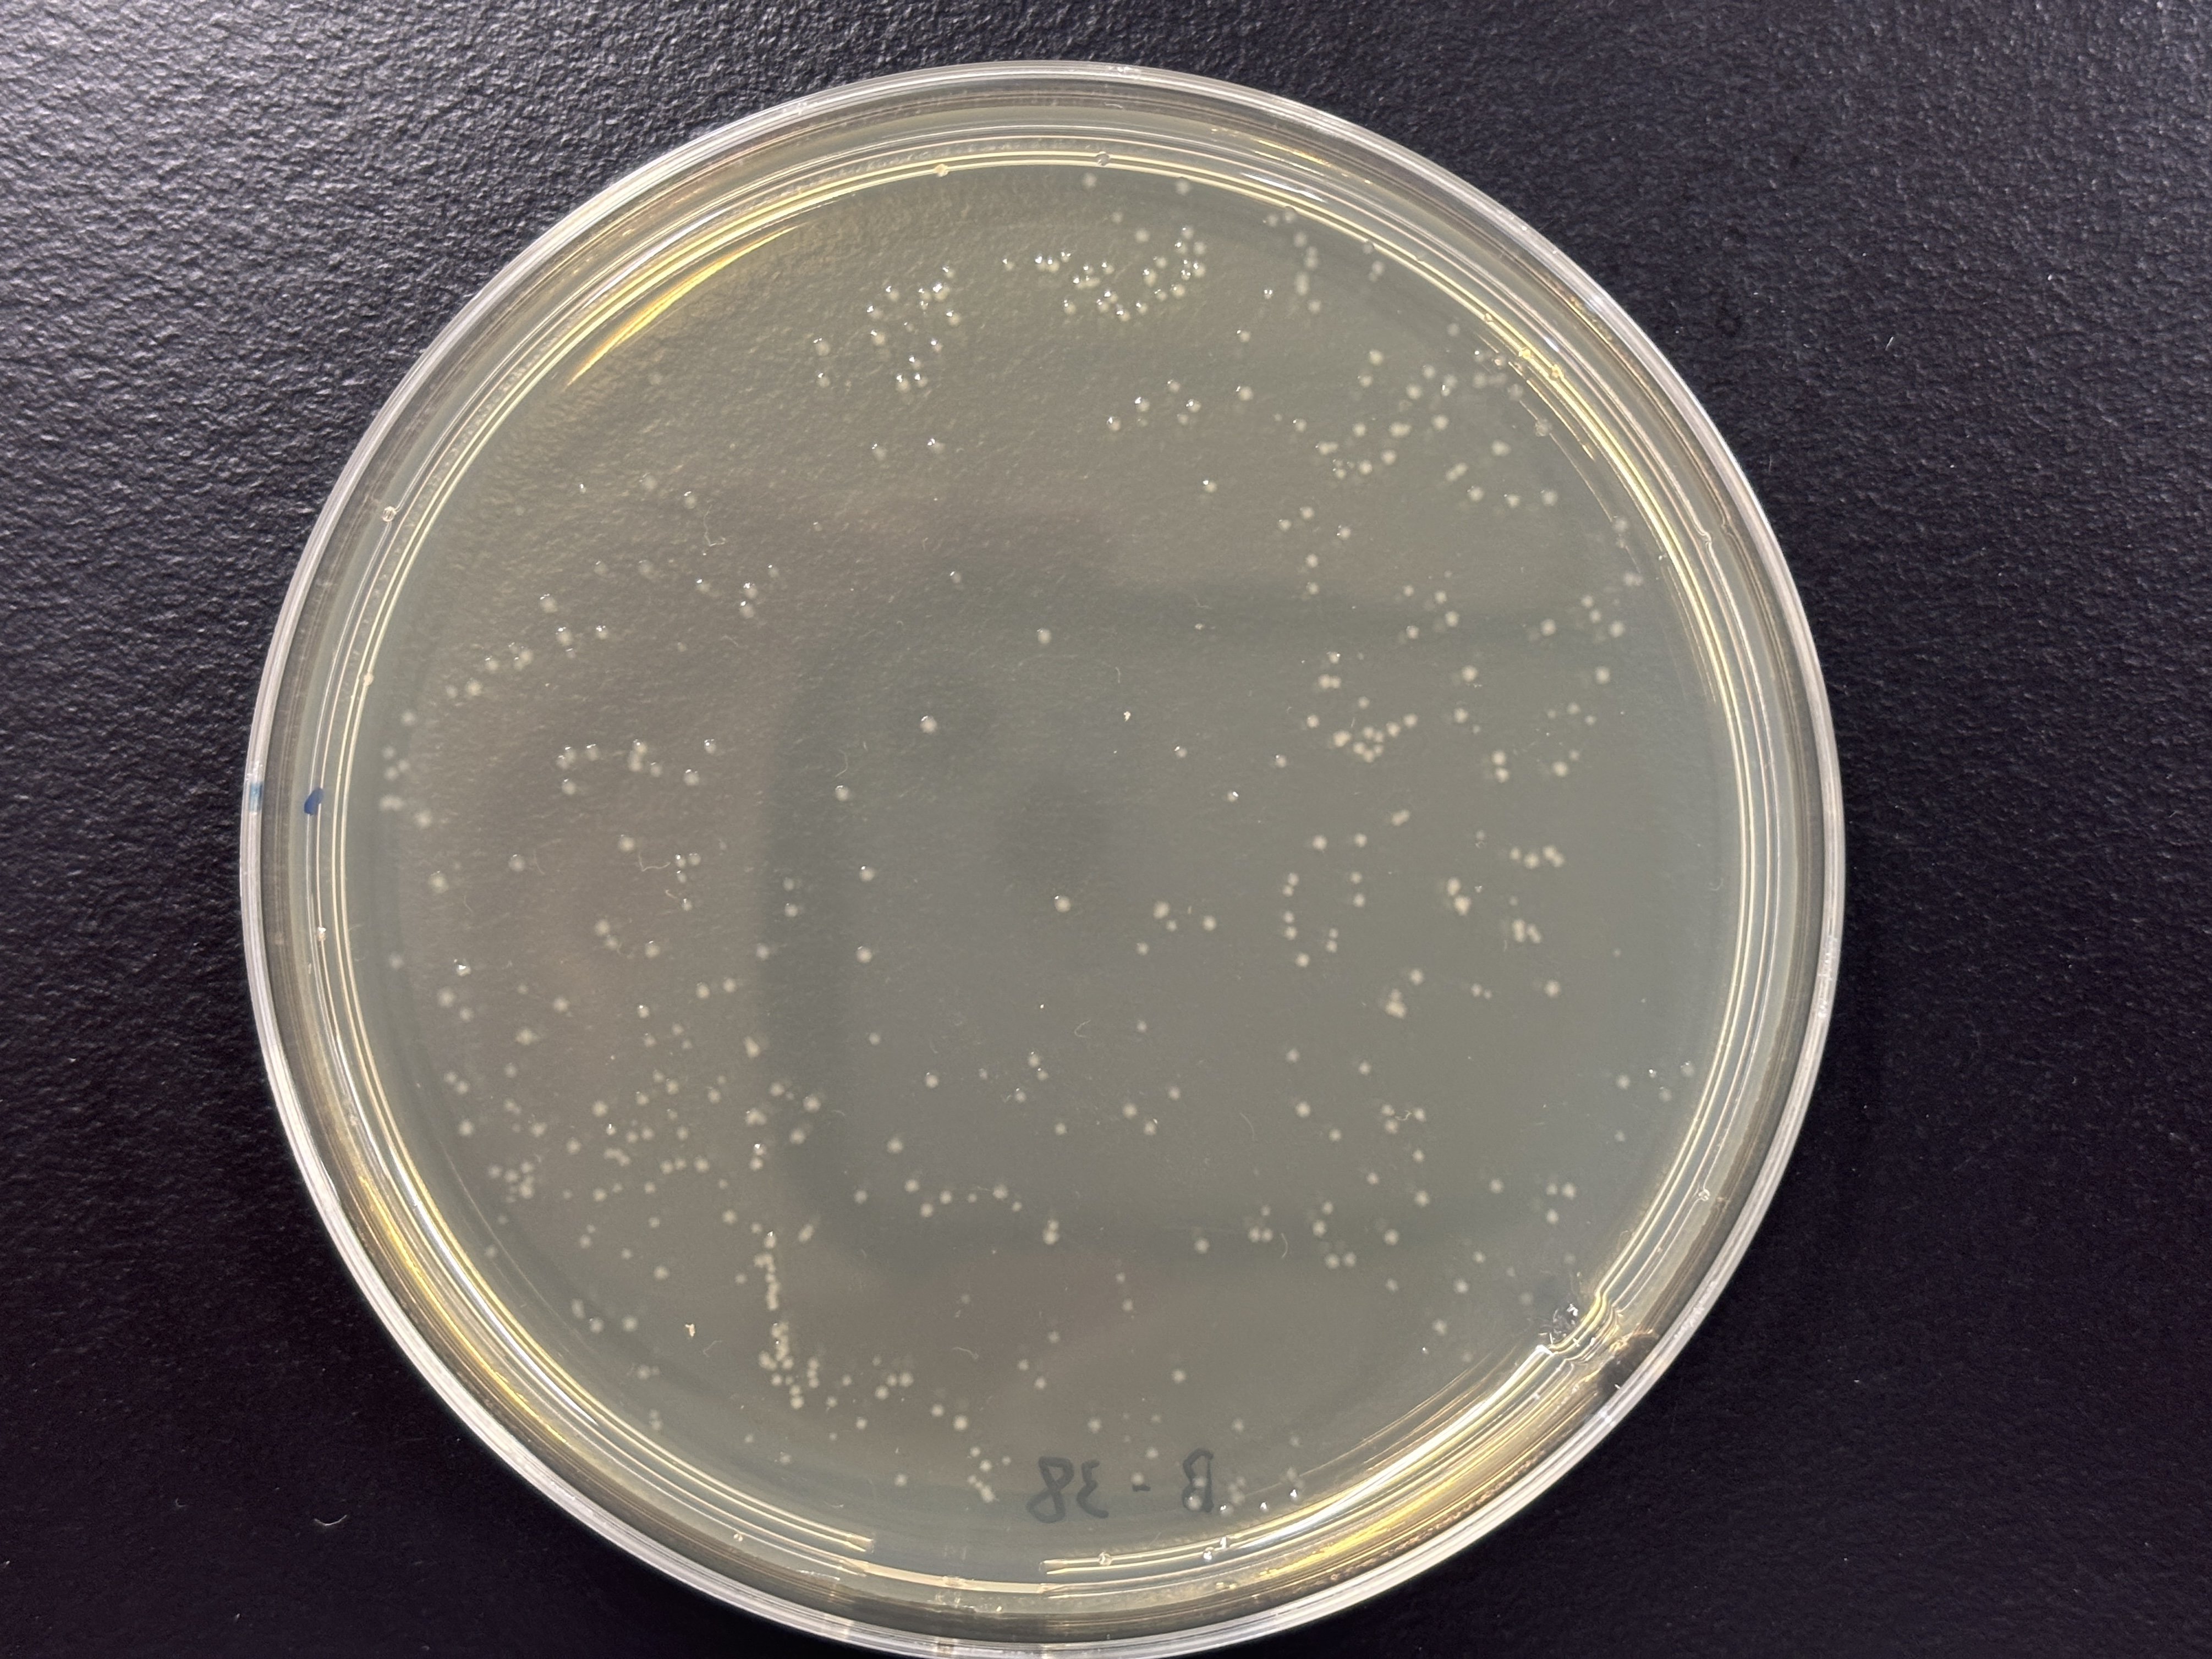
\includegraphics[width=\textwidth]{形質転換体コロニー_pBR322.jpg}
                    \caption{pBR322}
                    \label{fig:pBR322}
                \end{subfigure}
                \hfill
                \begin{subfigure}{0.49\textwidth}
                    \centering
                    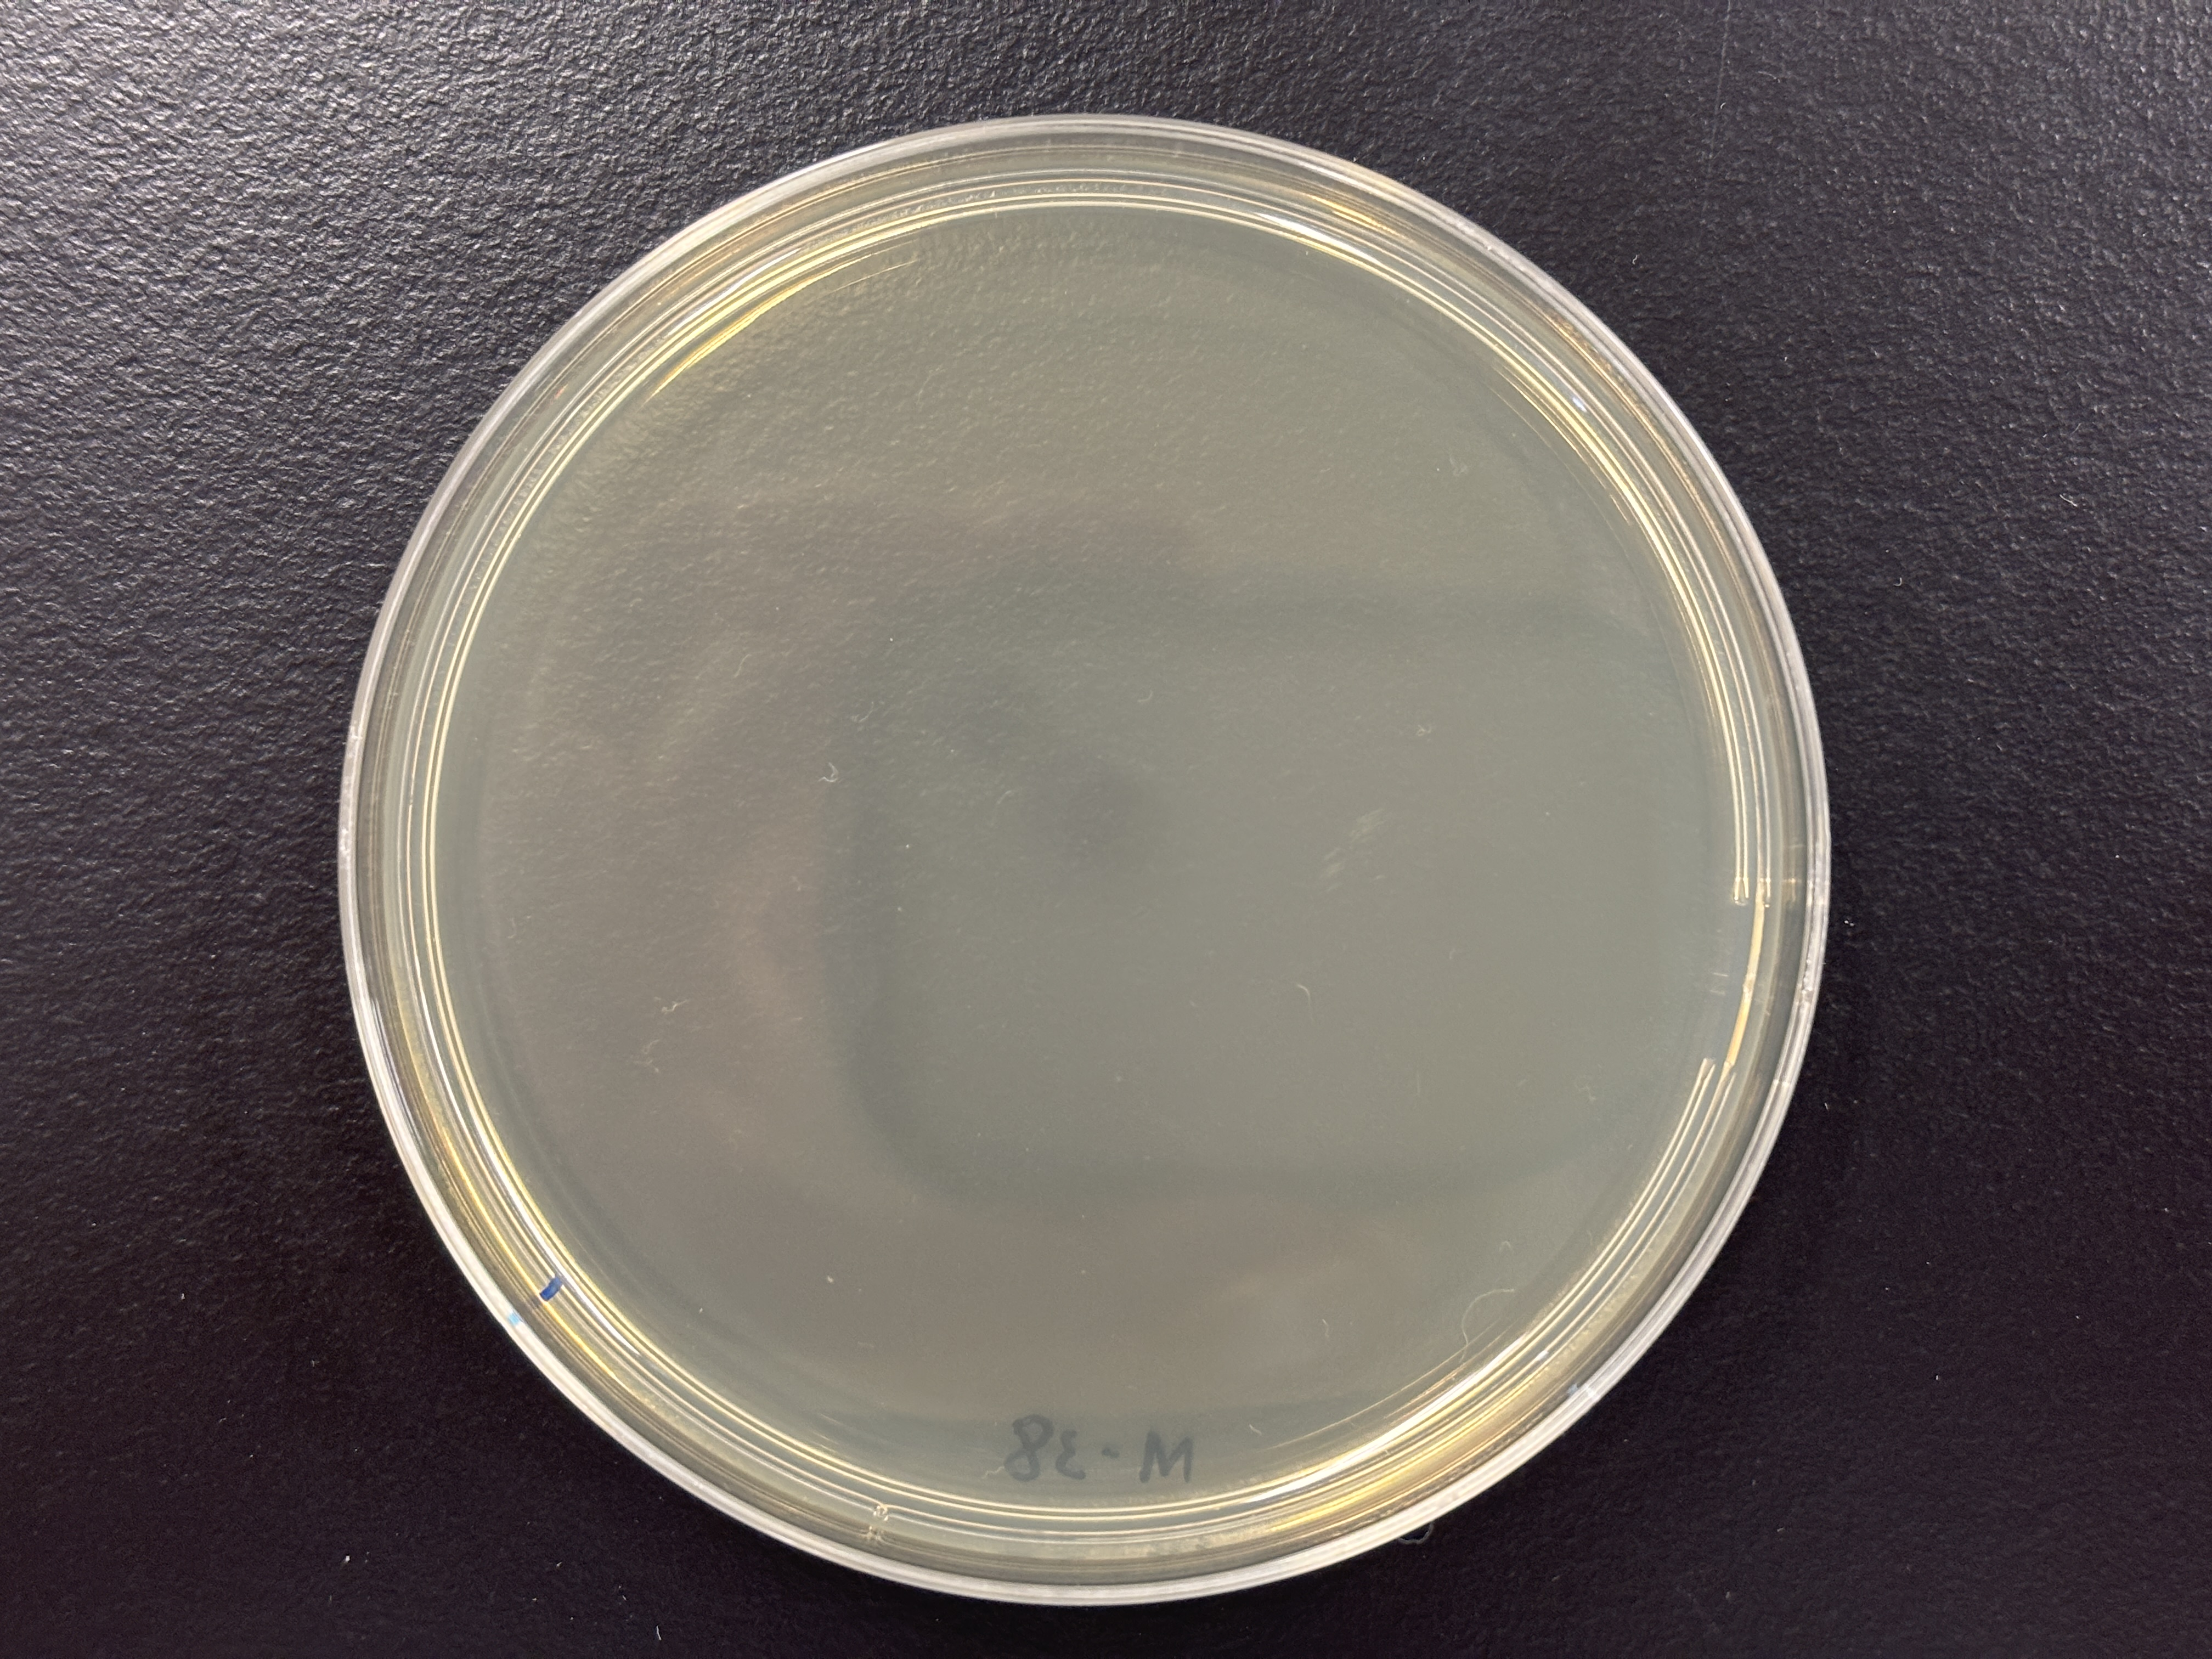
\includegraphics[width=\textwidth]{形質転換体コロニー_pMW118.jpg}
                    \caption{pMW118}
                    \label{fig:pMW118}
                \end{subfigure}
                \caption{カナマイシン含有LB寒天培地における各形質転換体の培養結果. \\
                (a) プラスミドpBR322を保有する大腸菌にpMWK1257を加えて形質転換させた菌体の培養結果. \\
                (b) プラスミドpMW118を保有する大腸菌にpMWK1257を加えて形質転換させた菌体の培養結果.}
                \label{fig:形質転換体}
            \end{figure}

            図\ref{fig:pBR322}より、プラスミドpBR322を保有する大腸菌の形質転換体のコロニー数は404個であった。また、図\ref{fig:pMW118}より、プラスミドpMW118を保有する大腸菌の形質転換体のコロニー数は0個であった。

            \subsubsection*{各形質転換体のコロニー数の解析}
                実習参加者全員の各形質転換体のコロニー数の平均値と標準偏差は以下の表\ref{tab:形質転換体}の通りであった。

                \begin{table}[H]
                    \centering
                    \caption{各形質転換体のコロニー数の平均値と標準偏差 ($n=41$)}
                    \label{tab:形質転換体}
                    \begin{tabularx}{\linewidth}{CCC}\toprule
                        形質転換体 & 平均値 $\bar{x}$ & 標準偏差 $s$ \\ \midrule
                        pBR322 / pMWK1257 & 699.73 & 619.60 \\
                        pMW118 / pMWK1257 & 0.19512 & 0.55765 \\ \bottomrule
                    \end{tabularx}
                \end{table}

                続いて、表\ref{tab:形質転換体}の値を用いて、プラスミドpBR322を保有する大腸菌の形質転換体のコロニー数と、プラスミドpMW118を保有する大腸菌の形質転換体のコロニー数に有意な差があるかどうかを解析する。
                
                表\ref{tab:形質転換体}より、実習参加者全員の標本におけるWelchのt統計量は
                \begin{align}
                    t = \frac{\bar{x}_1 - \bar{x}_2}{s_{\bar{x}_1 - \bar{x}_2}} = \cfrac{\bar{x}_1 - \bar{x}_2}{\sqrt{\cfrac{s_1^2}{n_1} + \cfrac{s_2^2}{n_2}}} \approx 7.2292
                \end{align}
                となった\cite{t-test}。ここで、$\bar{x}_1,\ \bar{x}_2$はそれぞれの形質転換体のコロニー数の平均値、$s_{\bar{x}_1 - \bar{x}_2}$は標準誤差(pooled SEM)、$s_1,\ s_2$はそれぞれの形質転換体のコロニー数の標準偏差、$n_1,\ n_2$はそれぞれの形質転換体のサンプル数であり、ここではどちらも41である。

                また、2標本の自由度$df$はWelch-Satterthwaiteの近似式より、
                \begin{equation}
                    df \approx \cfrac{\left( \cfrac{s_1^2}{n_1} + \cfrac{s_2^2}{n_2}\right) ^2}{\cfrac{s_1^4}{n_1^2 \cdot \nu_1} + \cfrac{s_2^4}{n_2^2 \cdot \nu_2}} = \cfrac{\left( \cfrac{s_1^2}{n_1} + \cfrac{s_2^2}{n_2}\right) ^2}{\cfrac{s_1^4}{n_1^2 \cdot (n_1 - 1)} + \cfrac{s_2^4}{n_2^2 \cdot (n_2-1)}} \approx 40
                \end{equation}
                となった\cite{t-test}。ここで、$\nu_1,\ \nu_2$はそれぞれの形質転換体ごとの標本の自由度であり、ここではどちらも$n - 1 = 40$である。

                以上より、「プラスミドpBR322を保有する大腸菌の形質転換体のコロニー数と、プラスミドpMW118を保有する大腸菌の形質転換体のコロニー数には有意な差が無い」と仮定する帰無仮説における両側p値は、
                \begin{equation}
                    p = 0.000000
                \end{equation}
                となった。これより、$p < 0.01$であるため、各形質転換体のコロニー数には有意な差があると言える。

        \subsection{プラスミドDNAの電気泳動結果}
            以下の図\ref{fig:電気泳動}に、2.3節において電気泳動したアガロースゲルの写真を示す。

            \begin{figure}[H]
                \centering
                \begin{subfigure}{0.49\textwidth}
                    \centering
                    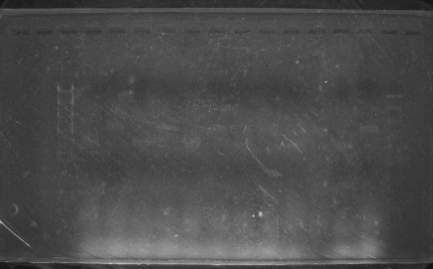
\includegraphics[width=\textwidth]{電気泳動_20min染色後.png}
                    \caption{20分間染色後}
                    \label{fig:電気泳動_20min染色後}
                \end{subfigure}
                \hfill
                \begin{subfigure}{0.49\textwidth}
                    \centering
                    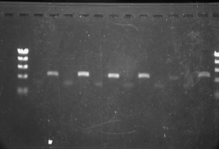
\includegraphics[width=\textwidth]{電気泳動_24h染色後.png}
                    \caption{24時間染色後}
                    \label{fig:電気泳動_24h染色後}
                \end{subfigure}
                \caption{大腸菌から抽出したプラスミドpMWK1257をEcoRIで制限消化したものと未処理のもので電気泳動し、ゲルを染色して紫外線イルミネーターで撮影したもの. \\
                (a) ゲルを20分間染色し、紫外線イルミネーターで撮影したもの. \\
                (b) ゲルをさらに24時間染色し、紫外線イルミネーターで撮影したもの.}
                \label{fig:電気泳動}
            \end{figure}

            図\ref{fig:電気泳動}において、青枠で囲ったレーンが$\lambda$HindⅢ分子量マーカーをアプライしたレーンであり、赤枠で囲ったレーンが本実験でプラスミドpMWK1257をアプライしたレーンである。また、赤枠で囲ったレーンのうち、左側が未処理のプラスミドpMWK1257、右側がEcoRI制限消化済みのプラスミドpMWK1257をアプライしたレーンである。

            図\ref{fig:電気泳動_20min染色後}では、分子量マーカーの薄いバンドが観察された。また、赤枠のレーンにおいて矢頭で示した高さ付近の上下に、それぞれ未処理のプラスミドと制限消化済みのプラスミドの薄いバンドが観察された。さらに、矢印で示したように、ゲルの下端には比較的濃い白いバンドが見られた。

            図\ref{fig:電気泳動_24h染色後}では、分子量マーカーの濃いバンドが観察された。各バンドの塩基対の長さは青枠で囲ったレーンの左側に示した通りである。赤枠で囲ったレーンでは、矢印で示したように、4.36 kbpほどの高さにEcoRI制限消化済みのプラスミドの濃いバンドが観察された。また、矢頭で示したように、2.32 kbpと4.36 kbpの中間ほどの高さに未処理のプラスミドの比較的薄いバンドが観察された。

    \section{考察}
        本節では、大腸菌の形質転換体においてコロニー数に有意な差が生じた理由、電気泳動において未処理のプラスミドと制限消化済みのプラスミドのバンドの移動度に違いが生じた理由について考察する。
        
        \subsection{大腸菌の形質転換体のコロニー数の違いについて}
            3.1節で述べたように、プラスミドpBR322を保有する大腸菌の形質転換体のコロニー数とプラスミドpMW118を保有する大腸菌の形質転換体のコロニー数には有意な差が見られた。このようなことが起こった原因として、形質転換体をカナマイシンが含まれる培地で培養したこと、そして、一方の形質転換体はカナマイシンに対して耐性を持ち、もう一方の形質転換体はカナマイシンに対して耐性を持たないことが考えられる。表\ref{tab:形質転換体}より、プラスミドpBR322を保有する大腸菌の形質転換体のコロニー数の平均値は約700であり、プラスミドpMW118を保有する大腸菌の形質転換体のコロニー数の平均値は0であった。したがって、プラスミドpBR322を保有する大腸菌の形質転換体はカナマイシン耐性を持つ一方で、プラスミドpMW118を保有する大腸菌の形質転換体はカナマイシン耐性を持たないと考えられる。

            本実験では、元々大腸菌が保有するプラスミド以外の条件が同じであるため、まず考えられることとして、プラスミドpBR322は大腸菌にカナマイシン耐性を付与するのに対し、プラスミドpMW118は大腸菌にカナマイシン耐性を付与しないことが挙げられる。しかし、プラスミドpBR322やpMW118はいずれもカナマイシン耐性遺伝子を持たない\cite{pBR322},\cite{pMW118}。本実験で用いたプラスミドのうち、カナマイシン耐性遺伝子を持つものはプラスミドpMWK1257のみである\cite{pHN1257}。
            
            以上のことから、プラスミドpBR322またはpMW118を保有する大腸菌をプラスミドpMWK1257によって形質転換した際、前者の細胞ではpMWK1257がpBR322と共存できたが、後者の細胞ではpMWK1257がpMW118と共存できなかった可能性が考えられる。このようなことが起こった原因として、プラスミドpMW118の複製起点とプラスミドpMWK1257の複製起点が同じであり、不和合性を示したことが挙げられる。このことは、プラスミドpMW118の複製起点がpSC101であり\cite{pMW118}、プラスミドpMWK1257の複製起点がpSC101$^\mathrm{H}$であること\cite{pHN1257}から説明できる。

            これらのことを踏まえると、本実験において形質転換体のコロニー数に有意な差が生じた理由として以下の説明が考えられる。プラスミドpBR322を保有する大腸菌はカナマイシン耐性遺伝子をもつプラスミドpMWK1257と和合性を示し、その形質転換体は新たにカナマイシン耐性を獲得した。一方で、プラスミドpMW118を保有する大腸菌はpMWK1257と不和合性を示し、その形質転換体はカナマイシン耐性を獲得しなかった。その結果、カナマイシンを含む培地中で前者の細胞は生き残ったが、後者の細胞は死滅したと考えられる。

        \subsection{未処理のプラスミドDNAと制限消化済みのプラスミドDNAのアガロースゲル電気泳動における移動度の違いについて}
            

    \section{課題}

    \begin{thebibliography}{9}
        \bibitem{t-test} Michael R Dohm. "10.2: Digging deeper into t-test plus the Welch test". LibreTexts\texttrademark \ STATISTICS, 2024. \url{https://stats.libretexts.org/Bookshelves/Applied_Statistics/Mikes_Biostatistics_Book_(Dohm)/10%3A_Quantitative_Two-Sample_Tests/10.2%3A_Digging_deeper_into_t-test_plus_the_Welch_test}, (閲覧 : 2026-11-1).

        \bibitem{pBR322} ニッポンジーン. "pBR322 DNA". \url{https://www.nippongene.com/siyaku/product/dna-cloning/pbr322-dna/pbr322-dna.html}, (閲覧 : 2026-11-2).

        \bibitem{pMW118} ニッポンジーン. "pMW118 DNA". \url{https://www.nippongene.com/siyaku/product/dna-cloning/pmw118-119-dna/pmw118-dna.html}, (閲覧 : 2026-11-2).

        \bibitem{pHN1257} Nobutaka Nakashima, Tomohiro Tamura. "Conditional gene silencing of multiple genes with antisense RNAs and generation of a mutator strain of \textit{Escherichia coli}". Nucleic Acids Research, 2009, Vol.37, No.15. \url{https://doi.org/10.1093/nar/gkp498}.
    \end{thebibliography}
\end{document}